\documentclass[tikz,convert={outfile=projection.svg}]{standalone}
\usepackage{graphicx} % Required for inserting images
\usepackage{tikz}
\title{projection drawings}
\author{Nathaniel Pritchard}
\date{October 2025}

\begin{document}

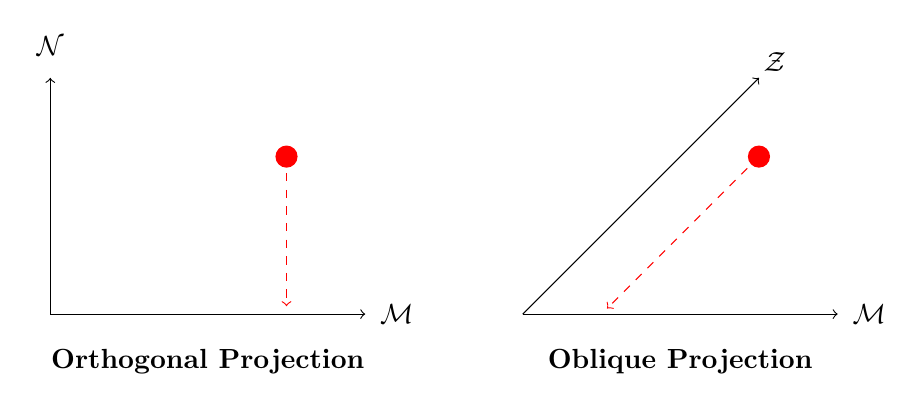
\begin{tikzpicture}[scale = 2]
    \draw[->] (0,0) -- +(0,1.5);
    \draw[->] (0,0) -- +(2,0);
    \fill[color = red] (1.5,1) circle(2pt);
    \draw[->, red, dashed, shorten >= 1mm] (1.5,1) -- +(0,-1);
    \node at (1,-.3) {\textbf{Orthogonal Projection}};
    \node at (0, 1.7) {$\mathcal{N}$};
    \node at (2.2, 0) {$\mathcal{M}$};
    
    \draw[->] (3,0) -- +(1.5,1.5);
    \draw[->] (3,0) -- +(2,0);
    \fill[color = red] (4.5,1) circle(2pt);
    \draw[->,red, dashed, shorten >= 1mm] (4.5,1) -- +(-1,-1);
    \node at (4,-.3) {\textbf{Oblique Projection}};
    \node at (5.2, 0) {$\mathcal{M}$};
    \node at (4.6, 1.6) {$\mathcal{Z}$};
\end{tikzpicture}

\end{document}

